\documentclass[12pt]{article}
 
\usepackage[T2A]{fontenc}
\usepackage[utf8]{inputenc}
\usepackage[bulgarian]{babel}
\usepackage{cite}
\usepackage{graphicx}
\usepackage{amsmath}
\usepackage{amsfonts}
\usepackage{float}
\usepackage{algpseudocode}
\usepackage{listings}
\usepackage[hidelinks]{hyperref}
\usepackage{pgfplots}
\usepackage{amssymb}
\usepackage{xcolor}

\definecolor{codegreen}{rgb}{0,0.6,0}
\definecolor{codegray}{rgb}{0.5,0.5,0.5}
\definecolor{codepurple}{rgb}{0.58,0,0.82}
\definecolor{backcolour}{rgb}{0.95,0.95,0.92}

\setlength{\parindent}{0ex}

\lstdefinestyle{mystyle}{
	backgroundcolor=\color{backcolour},
	commentstyle=\color{codegreen},
	keywordstyle=\color{magenta},
	numberstyle=\tiny\color{codegray},
	stringstyle=\color{codepurple},
	basicstyle=\ttfamily\footnotesize,
	breakatwhitespace=false,
	breaklines=true,
	captionpos=b,
	keepspaces=true,
	numbers=left,
	numbersep=5pt,
	showspaces=false,
	showstringspaces=false,
	showtabs=false,
	tabsize=2
}

\lstset{style=mystyle}

\graphicspath{{images/}}

\title{Изследване на скалируемостта на Wa-Tor симулацията при cтатично балансиране \\
	\large{Проект по курса ``Системи за паралелна обработка''}}

\author{Автор:\\ Иван-Асен Веселинов Чакъров \\
	ФН: 81837, Курс: 3, Група: 1}
\date{\today}


\pgfplotsset{compat=1.17}
\begin{document}

\maketitle

\newpage

\tableofcontents

\newpage

\section{Увод}
Wa-Tor~\cite{wator} е класически проблем при паралелното програмиране.
Накратко, задачата е симулирането на идеализиран двумерен свят с формата на тор.
Светът има два вида обитатели - херинги, които играят ролята на плячка и акули, които ловят и изяждат херингите.
\bigbreak
Декомпозицията на домейнa (Domain decomposition)~\cite{domain_decomposition}
при паралелното програмиране се явява естествен подход при решаването на проблеми,
при които за решаването на проблема за даден елемент $D$ от домейна са нужни само малко подмножество от данни,
които са "близо" до $D$. Накратко, идеята е, че разбиваме домейна на множество поддомейни
и възлагаме решаването на проблема за всеки поддомейн на отделен процес.
Важно е отделните поддомейни да са със сравнително еднаква големина за да може да се разпредели
равномерно работата между процесите. Съществуват два вида декомпозиция - статична и динамична.
При статичната в началото на алгоритъма разбиваме домейна и разпределяме работата между процесите.
По време на симулацията разбиването не се променя, което може да води до намаляване на производителността,
тъй като данните при доста алгоритми прескачат от един поддомейн в друг и това може да доведе до дисбаланс
на работата, която даден процес трябва да извърши. Този проблем се решава от динамичната декомпозиция, която по време на симулацията
преизчислява разбиването на домейна с цел балансиране на големината на отделните поддомейни.
Декомпозицията на домейни намира приложение при решаването на проблеми от тип Cellular automata ~\cite{cellular_automata}.
\bigbreak
Тъй като и Wa-Tor попада в този тип проблеми, представеното решение тук е базирано
на статична декомпозиция на домейна.

\newpage
\section{Правилата на света Wa-Tor}

Светът на Wa-Tor се намира на повърхността на Тор (или поничка).
Цялата повърхност е покрита с вода и единствените обитатели на този свят са
херингите, които играят ролята на плячка и акулите, които ловят плячката.
Позициите, които заемат рибите cа дискретни и могат да се изобразят с
двумерна матрица. Времето тече под формата на дискретни итерации, като на всяка
итерация дадена риба променя позицията си, изяжда друга риба, умира или ражда
нова себеподобна риба. Точните правила, по които това става са следните:

\bigbreak
\textbf{Движение}:
\begin{itemize}
	\item Херинга: Избира случайна съседна (горна, долна, лява или дясна) свободна клетка и се премества в нея.
	\item Акула: Избира случайна сеседна клетка с херинга в нея и ако намери такава се мести там и изяжда херингата,
		а ако няма съседна клетка с херинга се мести на случайна съседна клетка. 
\end{itemize}

\textbf{Умиране}:
\begin{itemize}
	\item Херинга: При нашата имплементация херингите са безсмъртни. Единственият начин да умрат е ако бедат изядени
		от акула. В такъв случай биват изтрити от Света. Възможно е да се направи вариант, в който да имат краен живот,
		в който на всяка итерация губят по една точка енергия и ако стане тя 0 - умират.
	\item Акула: На всяка итерация ако не изяде някоя херинга губи по една точка енергия. Ако енергията стане 0
		умира и бива изтрита от света на Wa-Tor. Ако изяде херинга на дадена итерация и се добавя една точка енергия.
\end{itemize}

\textbf{Размножаване}:
\\
Еднакво за всички риби. Всяка риба има възраст - число, което започва от 0 при раждане и на всяка итерация
се увеличава с 1. Когато дадена риба стигне "максималната възраст" и се нулира възрастта и на старата и позиция се създава нова
риба от същия тип (херинга или акула), която е с възраст 0. Възможно е "максималнатa възраст" да е различна за акулите и херингите.

\bigbreak
В интернет има най-различни разновидности на тези правила. Най-вероятно това е, защото в първоизточникът ~\cite{wator}
правилата не са описани особено формално описани и, защото много различни имплементации си добавят или променят правила.
Има варианти на симулацията, в които и херингите се хранят - с планктон примерно. Нашата имплементация, обаче
е базирана на горе описаните правила и изследва скалируемост спрямо тях.

\section{Инструкции за употреба на проекта}
Програмата се разпространява по 2 основни начина:

\begin{itemize}
	\item Linux container (Docker): В този вид програмата носи със себе си всички неща на които зависи.
		За да се пусне на дадена машина трябва да има инсталиран Docker. Това е и използваният начин
		за изкарването на тестовите резултати.
	\item Java JAR: Стандартен начин за разпространие на Java базирани програми. Особеност е, че проектът
		е разработен на Java 16, като използва и експериментални функции на езика, така че
		препоръчаният начин за използване е през Linux container-a.
\end{itemize}

\bigbreak

Примерни команди в Bash за пускане на програмата:

\begin{lstlisting}[language=Bash, caption=Пускане на програмата през Docker]
docker run -e ARGS='
	$threads \
	$iterations \
	$sharks \
	$fish \
	$height \
	$width' \
	ivanasen-wator:0.0.1
\end{lstlisting}

\begin{lstlisting}[language=Bash, caption=Пускане на програмата директно през Java]
java -jar ivanasen-wator.jar \
	$threads \
	$iterations \
	$sharks \
	$fish \
	$height \
	$width
\end{lstlisting}

\bigbreak

Значение на аргументите:
\begin{itemize}
	\item \$threads: Брой нишки
	\item \$iterations: Брой итерации, през които да мине симулацията
	\item \$sharks: Брой акули
	\item \$fish: Брой херинги
	\item \$height: Височина на полето
	\item \$width: Широчина на полето
\end{itemize}

\bigbreak

Пример за резултатът от изпълнението, който се изкарва на стандартния изход:

\begin{lstlisting}[language=Bash]
NThreads: 1
Iterations: 100
Shark count: 10000
Fish count: 1000000
Height: 6000
Width: 3000
Execution time millis: 400143
\end{lstlisting}

Интересният ред е Execution time millis - времето за изпълнение в милисекунди прекарано
изпълнявайки симулацията от началото на работата на първата $Worker$ нишка до края
на изпълнението на последната. Повече за $Worker$ нишките обясняваме във следващата секция.

\newpage

\section{Описание на паралелния алгоритъм}
Алгоритъмът, който позлваме се базира на статична декомпозиция на домейна.
Начинът, по който работи е следният. Да кажем, че искаме да изпълним алгоритъма с N на брой нишки.
Разбиваме полето на $N$ на брой непрекъснати участъка (поддомейна) по редове като гледаме големината им
по възможност да е еднаква. Ако височината $H$ не се дели точно на $N$ прибавяме остатъка към последния поддомейн.
След това възлагаме всеки поддомейн на отделна нишка, която си изчислява симулацията само за него.
Друг подход за разбиване би бил по "правоъглници" , тоест да имаме по няколко поддомейна на ред.
Изборът да го направим по редове е по 2 причини. Едната е, че така всеки поддомейн си комуникира само
с 2 съседа вместо с 4, което намалява времето за комуникация между отделните нишки, а втората причина
е, че този алгоритъм е по-прост за реализация.
\bigbreak
След като сме разпределили поддомейните на нишките начинът, по който те си синхронизират работата е следния.
Всяка нишка обработва своя участък по редове, като започва от най-горния. След като го обработи изпраща
съобщение, че е свършила работа по него на нишката, която отговаря за съседния горен участък.
След това обработва вътрешните си редове без да праща никакви съобщения на никого, подобно на еднонишкова
имплементация. Преди да стигне най-долния ред изчаква да получи съобщение от нишката отговаряща за съседния
долен участък, че си е свършила работа по нейния пръв ред. След като го е получила завършва с обработката
и на последния ред. Така завършва една итерация от Wa-Tor симулацията за една нишка. След това нишката
продължава със следващата итерация, пак започвайки от първия ред.

В нашата имплементация на този алгоритъм използваме нишки на ниво операционна система, семафори и споделена памет за комуникация.
На следващата страница представяме с псевдокод стъпките, които изпълнява една нишка за една итерация.

\newpage

Нека $rowMutex[i]$ е семафор с начална стойност 1 за $i \in 1...H$.
Този семафор играе ролята на мютекс за достъп до даден ред на полето с номер $i$.
Нека $isUpdated[i]$ е семафор с начална стойност 0 за $i \in 1...H$.
Отново тези семафори са номерирани по редовете на полето. Служат за уведомяване,
че първия ред от участъка на дадена нишка е обработен.
Нека $startRow$ и $endRow$ са съответно номера на първия и последния ред,
който дадена нишка трябва да обработи.
\medbreak
\begin{algorithmic}
\For{$i\gets startRow; i \leq endRow; i\gets i + 1$}
	\State $nextRow\gets (i + 1) \mod H$
	\If {$i = startRow$}
		\State \Call{Acquire}{$rowMutex[i]$}
	\ElsIf{$i = endRow$}
		\State \Call{Acquire}{$isUpdated[nextRow]$}
		\State \Call{Acquire}{$rowMutex[nextRow]$}
	\EndIf

	\State \Call{UpdateStateForRow}{$i$}

	\If {$i = startRow$}
		\State \Call{Release}{$rowMutex[i]$}
		\State \Call{Release}{$isUpdated[i]$}
	\ElsIf{$i = endRow$}
		\State \Call{Release}{$rowMutex[nextRow]$}
	\EndIf
\EndFor
\end{algorithmic}
\medbreak
Както виждаме този псевдокод е по-формална версия на алгоритъма, който описахме с думи.

Друго интересно нещо при алгоритъма ни е начинът по който представяме двумерния свят, в който се намират
обитателите на Wa-Tor. Освен, че използваме двумерна матрица за представянето на клетките
имаме и масив от свързани списъци от класа Creature, който представлява обитателите на даден
ред от полето. Тоест ако искаме да обработим даден ред ние трябва да итерираме свързания списък.
Това спестява много посещения на празни клетки, които имплементацията само със двумерна матрица прави.

Цялостно, алгоритъмът като имплементация е подобен на този във ~\cite{bounded_neighbours}, но е опростена
версия, тъй като използва статична декомпозиция на домейна, т.е. не правим никакво балансиране на тежестта
по време на изпълнение и само разбиваме домейна в началото.

\newpage

\section{Архитектура}
Решението е имплементирано на Java 16 и използва вградените способности за паралелно програмиране
използвайки нишки и споделена памет:
\begin{itemize}
	\item Thread: Класът за нишка в Java
	\item ExecutorService: Упрявлява множество нишки в даден Thread pool
	\item ReentrantLock: Мютекс
	\item Semaphore: Семафор
\end{itemize}

Важно е да отбележим, че при имплементацията на JVM, която ползваме (OpenJDK 16) нишките са истински
на ниво ядро на операционната система, тъй като има стари версии на JVM и нови разработки като Project Loom~\cite{loom},
при които се използва тъй наречения Green Thread модел, при който нишките се менежират от самата JVM 
и позволяват мултиплексиране на много JVM нишки върху една ОС нишка.
\bigbreak
Архитектурата на проекта е направена по модела Master-Slaves, тъй като имаме една главна нишка,
която управлява множество Worker нишки, които извършват изчисленията необходими за симулацията.
\bigbreak
Ще отбележим по-важните класове на програмата:
\begin{itemize}
	\item Creature (и наследниците му Fish и Shark): В Creature е общата логика за това как се държи
		даден обитател в нашия свят. Fish и Shark съдържат специфичните правила, по които се движат
		по полето.
	\item State: Представлява имплементацията за състоянието, в което се намира нашия свят.
	\item Worker: Този клас имплементира Runnable. Той представлява кода, който се изпълнява от една нишка
		върху даден участък от света. Инстанциите на класа играят ролята на slaves в нашия модел.
	\item World: Този клас играе ролята на Master. В него се съдържа логиката за създаването и управлението на отделните
		Worker-и използвайки ExecutorService.
	\item Simulation: Създава World и мери времето за изпълнение на N на брой итерации на State.
	\item GuiSimulation: Създава World и показва в графичен вид в реално време как тече симулацията.
		Тук използваме Java Swing и AWT за целта.
\end{itemize}

На следващата страница представяме UML клас диаграма на проекта.

\newpage

\begin{figure}[H]
	\centering
	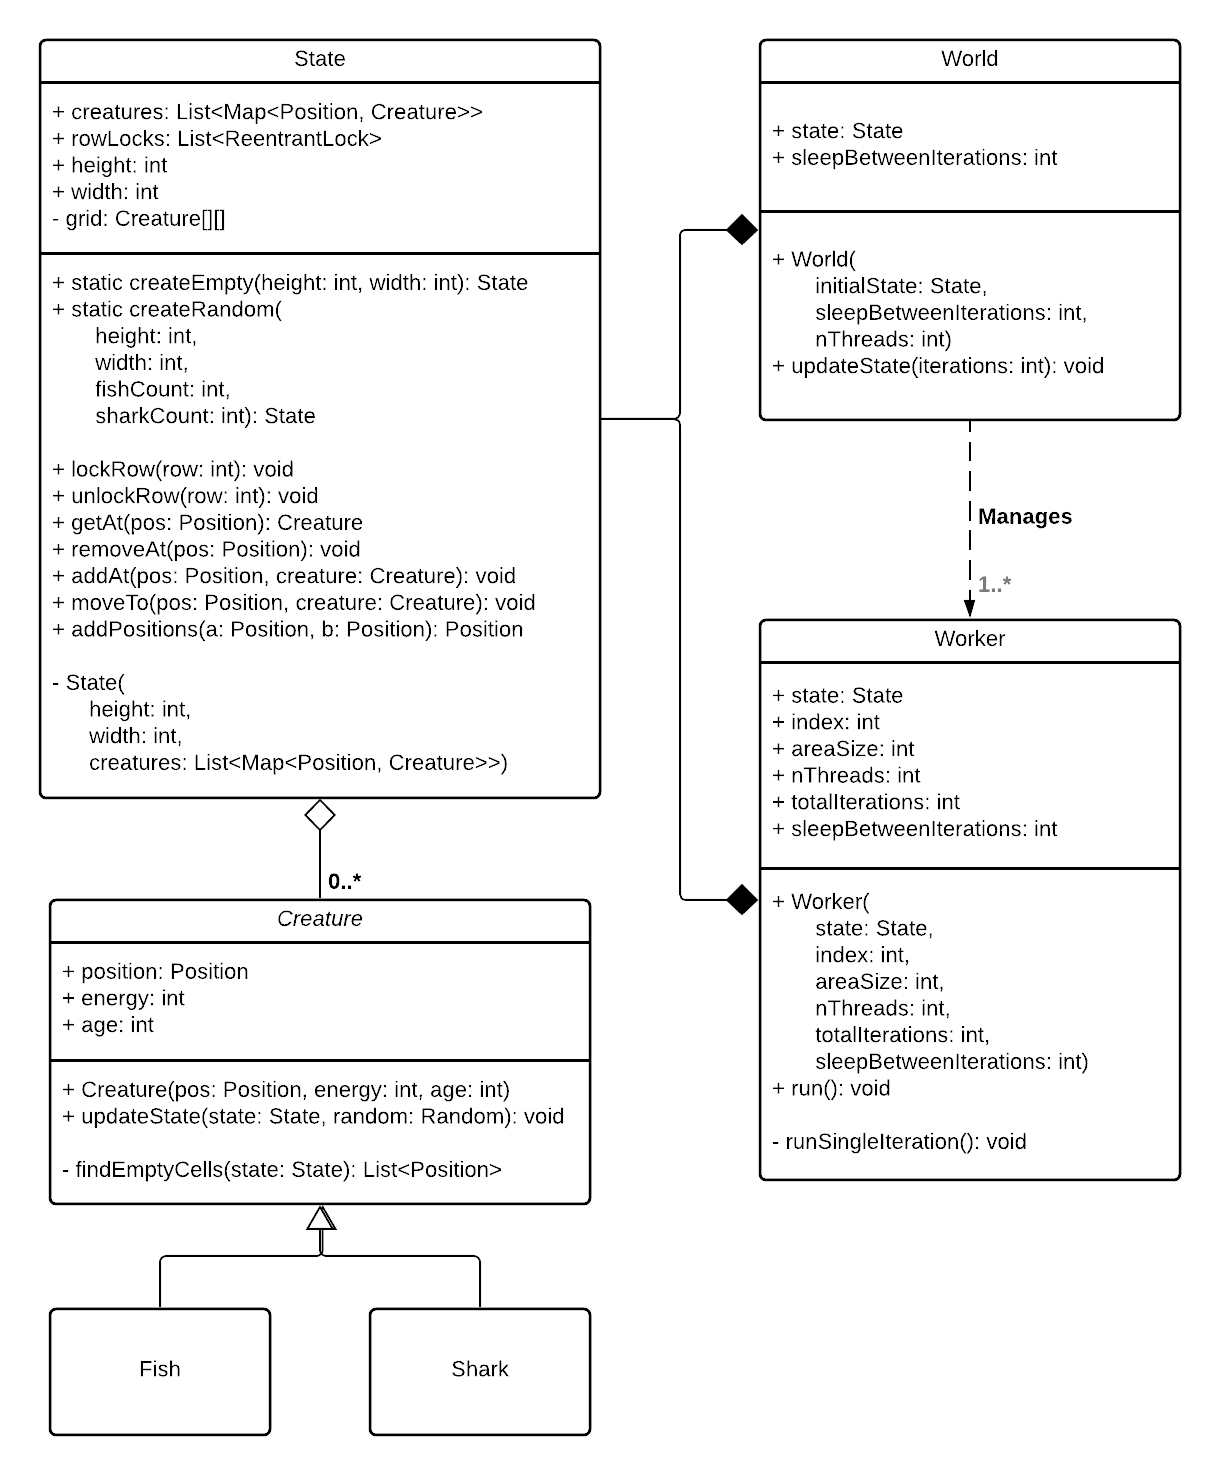
\includegraphics[width=1.2\textwidth]{classes-uml.png}
	\caption{UML Клас диаграма на проекта}
\end{figure}

\newpage

Хубаво е да знаем и начинът, по който тези класове си взаимодесйтват по време на изпълнение на приложението.
По тази причина показваме и UML Sequence диаграма.

\begin{figure}[H]
	\hspace*{-4cm}
	\centering
	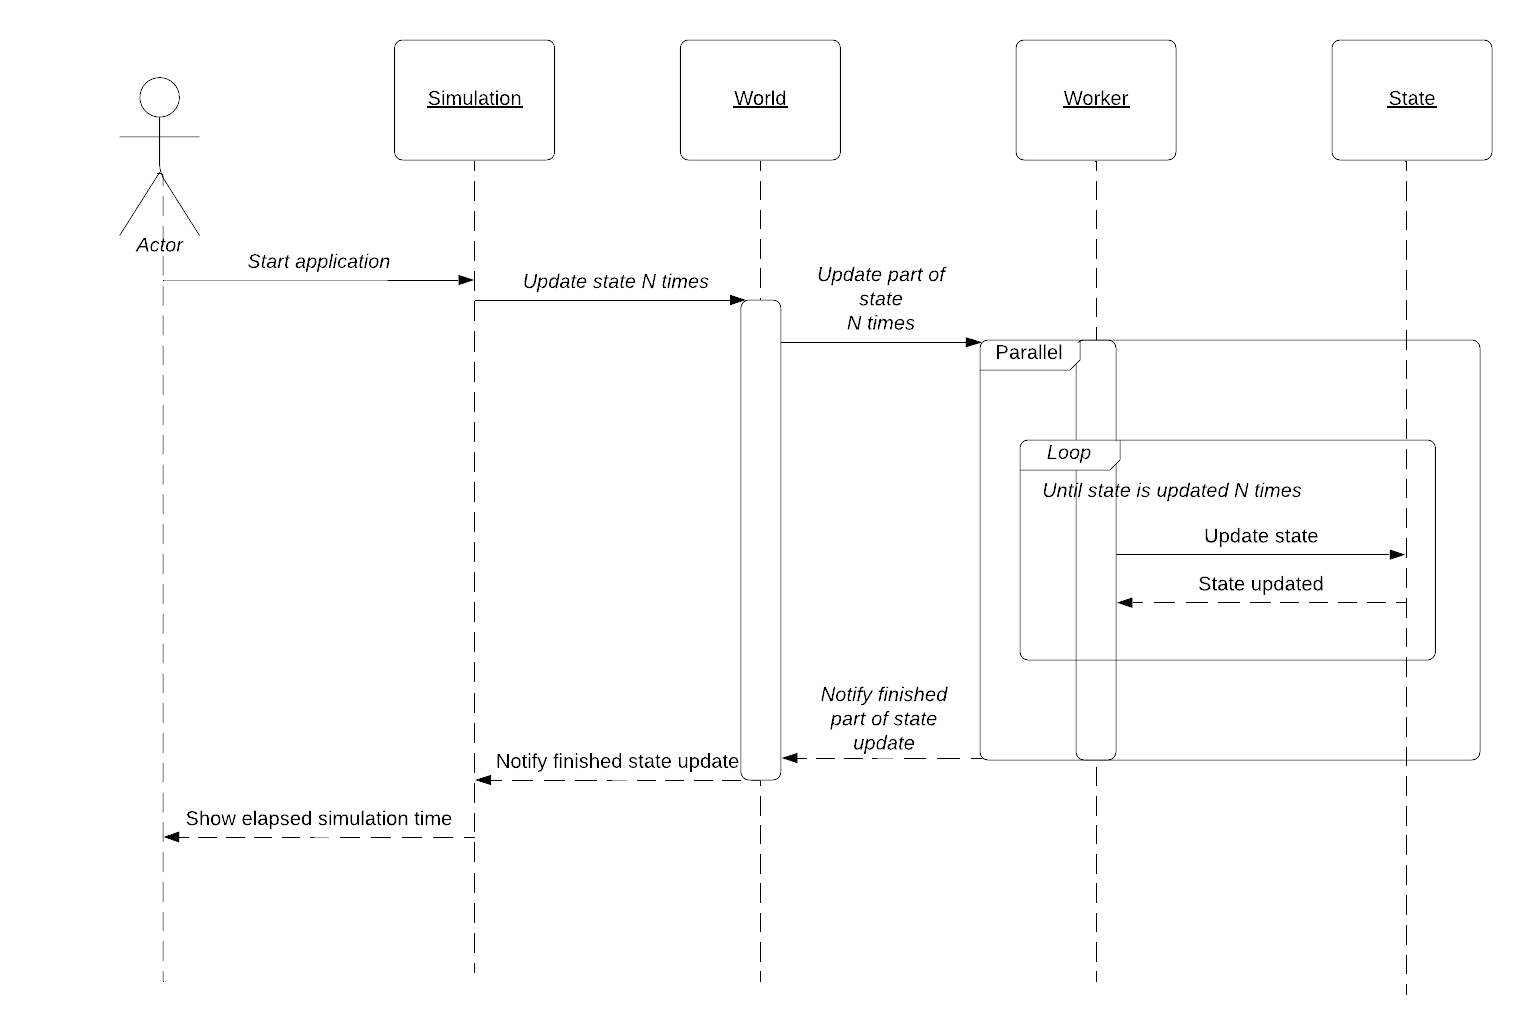
\includegraphics[width=1.5\textwidth]{sequence.png}
	\caption{UML диаграма на последователностите на проекта}
\end{figure}

\newpage
Разказано с думи това, което се случва по време на изпълнение е следното. Изпълнението започва с класа Simulation,
тъй като в него е main метода за Java. Първоначално той си създава инстанция на State, която е със случайно
разпределение на рибите из полето. След това създава и World обект, като му подава State. Първоначалното
създаване на графа на обекти в приложението не е изобразен на Sequence диаграмата, тъй като не е част от основния
алгоритъм, който се опитваме да паралелизираме. Всички описани неща до сега се случват последователно на
Main нишката на JVM. След това Simulation пуска заявка на World да се ъпдейтне за N итерации, като преди това
започва и измерване на времето за изпълнение. World след това, използвайки ExecutorService пуска $p$ на брой
нишки, като ги разпределя всяка да работи на отделен последователен брой от редове от полето. Всяка нишка
обработва своята част от полето за $N$ итерации, като същевременно си комуникира и се синхронизира със своите
съседи. След като всички нишки завършат работа World разбира това благодарение а ExecutorService-a и
връща резултат на Simulation, че е завършила своята работа. Simulation след това измерва точно колко време
е минало от момента, в който е дал заявка на World да направи симулацията до момента в който е получил
резултат и изкарва полученото време в милисекунди на стандартния изход (stdout).
\bigbreak
Правилата на които е базиран Wa-Tor ни принуждават да използваме генератори на случайни числа при всеки избор на това
в каква посока трябва да се придвижи дадена риба. По тази причина за да намалим недетерминистичното поведение
и да получим по-предвидими тестови резултати изполваме винаги детерминистичен seed за всички създаващи се инстанции
на Random класа в Java. Всяка нишка си има отделна инстанция, която се инициализира със seed равен на номера на самата нишка.
По принцип в случаи, в които искаме да генерираме случайни числа от много нишки е хубаво да се използва
обект от класа ThreadLocalRandom, който се споделя от различните нишки. Така споделяме обекта и единствено
началния seed за всяка нишка е различен. Това е по-добре от използване на цял нов обект за всяка нишка,
но в нашия случай искаме да имаме детерминистичен seed за всяка нишка, а във ThreadLocalRandom няма 
как да се специфицира началния seed, който искаме да ползваме. Затова просто използваме отделни инстанции
на Radnom класа.

\newpage

\section{Анализ}

Характеристики на тестовата машина: 
\begin{itemize}
	\item Процесор: 2 x Intel® Xeon® CPU E5-2660 0 @ 2.20GHz - Всеки процесор е с по 8 ядра и 2 нишки,
	това прави 16 ядра общо и 32 нишки (по 2 нишки на ядро благодарение на Hyperthreading).
	\item Памет: 64Gb, 32K L1d и L1i кешове, 256K L2 кеш и 20480К L3 кеш
\end{itemize}
Взимайки в предвид броя на нишките на машината има смисъл да тестваме скалируемост с до 32 паралелно работещи нишки.
Не очакваме, обаче след като минем брой на нишките да ни е 16 да получаваме особено добро подобрение в производителността,
тъй като 16 процесора с Hyperthreading изобщо не заместват 32 процесора.
\bigbreak
Начинът по, който са получени резултатите е следният. Пускаме симулацията да върви за $N$ итерации
и засичаме времето от началото на работата на първата $Worker$ нишка до края на работата на последната.
Правим отделни измервания от 1 до 32 нишки (не за всеки възможен брой, от съображения за
спестяване на време), като правим по 5 за всеки $K$ на брой нишки. След това
взимаме най-добрите резултати от тези 5 теста в получените графики тъй като приемаме, че всякакво забавяне е резултат от
"шум", който се въвежда от работата не други процеси на машината. Най-малкото последните дни преди края
на срока за предаването на проектите доста от студентите тестваха на машината и беше трудно да се уцели
момент, в който никой друг не тества.
\bigbreak
Като грануларност сме тествали единствено с $g = 1$. Подзадачите при нас са подполетата, на които е разбито голямото поле.
Ако броят на подполетата, на които разбиваме полето е $N$, а имаме $p$ нишки, то $g = N/p$ ни е грануларността.
Причините да няма смисъл да тестваме $g > 1$ са 2. Едната е, че разпределението на тежестта в отделните поддомейни
при Wa-Tor е много динамичнa, т.е. броя на рибите които се намират в отделните поддомейни се мени постоянно и дисбалансът,
който е получен се мени посотянно и много бързо. Така, че даже да разбием полето на повече части от броя процеси и да
разпределим работата им по отделните поддомейни спрямо броя риби, всякакви печалби от това ще траят няколко итерации.
Втората причина е самата природа на езика Java и това, че използваме непримитивни обекти за представянето на рибите.
Както знаем, Java слага всички такива обекти на Heap-а и нямаме никакви гаранции за data locality дори да имаме масив.
Единствено референциите към тези обекти ще се намират едни до други. Та, затова сме се ограничили само до $g = 1$.
Един възможен начин да се борим с дисбаланса на тежестта, който се мени динамично е пак да използваме статична декомпозиция на домейна,
т.е. разбиваме полето на $N$ подполета в началото и големината им седи константна по време на симулацията и ако изберем $p < N$ можем да разпределяме
по някакъв алгоритъм за балансиране на тежестта подполетата, които дадена нишка има да изчисли на всяка итерация.
Да вземем пример: Да кажем, че сме разбили полето на 2 части по редове и 99\% от рибите се намират в долната половина
на полето. При $g = 1$, както сме го имплементирали ние първата нишка ще пресметне много бързо нейната половина, докато
втората ще смята ~ 99\% от времето, а през това време първата няма да прави нищо. Ако го направим с $g = 2$ обаче
т.е. да разбием полето по редове на 4 части и отново да имаме 2 нишки, е възможно 2-те да работят първо по долните 2
реда и след това да обработят първите 2. Най-простия начин това да стане е да дистрибутираме
работата по отделните "гранули" по псевдослучаен начин. Вторият начин да се борим с този проблем е да променяме големината
на поддомейна, който дадена нишка има да обработи. При горния пример вместо да имаме 1\% от работата само за
горната половина от полето можем да увеличим големината на този поддомейн да стига например до 3/4 от височината погледнато
отгоре надолу. Втората нишка работи единствено по последната 1/4. Така отново постигаме динамично балансиране на тежестта и за разлика
от разбиването на гранули тук не увеличаваме времето за комуникация между отделните нишки.
Пример за такъв алгоритъм със динамична декомпозиция на домейна е Bounded neighbours ~\cite{bounded_neighbours}.
\\
Да отбележим, че началните позиции, които рибите заемат на полето са равномерно разпределни. В такива случаи е близо до
невъзможно да се получи такъв дисбаланс в началото подобен на гореописания (поне за големи полета). По тази причина
и разбиването на работата в началото я правим по равен брой редове на нишка, а не спрямо броя на рибите, които има в даден
поддомейн.
\\

\section{Тестови резултати}

\bigbreak
Изледвали сме скалируемостта при 2 различни набора от параметри:
\begin{itemize}
	\item $height = 2000, width = 1000, iterations = 200, sharks = 5000, fish = 50 000, \# = 10$
	\item $height = 4000, width = 2000, iterations = 50, sharks = 100 000, fish = 1 000 000, \# = 10$
\end{itemize}

Идеята да тестваме и при по-голямо поле е да видим как промяната на големината на данните
влияе на ускорението. Това, което очакваме е то да е по-добро при по-голямо поле с повече риби.
Тъй като пропорционално времето нужно за менежирането на нишките и времето за комуникация между тях
е по-малко.

\bigbreak

Следват таблици с резултатите, които сме получили при тестване.

\bigbreak
Значение на таблицитете с резултатите, които сме получили от тестване:
\begin{itemize}
	\item \#: Номер на теста
	\item $p$: Брой нишки
	\item $T^{(i)}_p$: Времето за изпълнение в милисекунди за i-тия тест за p нишки. $i \in 1..5$
	\item $T_p = min(T^{(i)}_p)$
	\item $S_p = T_1 / T_p$
	\item $E_p = S_p / p$
\end{itemize}
\newpage

\begin{tabular}{ |p{0.6cm}||p{1cm}|p{1cm}|p{1cm}|p{1cm}|p{1cm}|p{1cm}|p{1cm}|p{0.9cm}|p{0.9cm}| }
 \hline
 \multicolumn{10}{|c|}{Тестове при размер на полето 1000x2000 и популация 50 000} \\
 \hline
 \# & $p$ & $T^{(1)}_p$ & $T^{(2)}_p$ & $T^{(3)}_p$ & $T^{(4)}_p$ & $T^{(5)}_p$ & $T_p$ & $S_p$ & $E_p$ \\
 \hline
1  & 1  & 87521 & 85238 & 88839 & 88392 & 83791 & 83791 & 1.00 & 1.00 \\
2  & 2  & 43636 &  43001 & 42122 & 42790 & 42451 & 42122 & 1.98 & 0.99 \\
3  & 4  & 23608 & 23848 & 23023 & 21739 & 23980 & 21739 & 3.85 & 0.96 \\
4  & 8  & 15380 & 15380 & 17515 & 17541 & 22925 & 15380 & 5.44 & 0.68 \\
5  & 12 & 12934 & 10676 & 10307 & 9834 & 9906 & 9834 & 8.52 & 0.71 \\
6  & 16 & 9089 & 9315 & 9004 & 9134 & 9245 & 9004 & 9.31 & 0.58 \\
7  & 20 & 8826 & 9019 & 8913 & 9056 & 9033 & 8826 & 9.49 & 0.47 \\
8  & 24 & 8716 & 8628 & 9207 & 9010 & 8833 & 8628 & 9.71 & 0.40 \\
9  & 28 & 9462 & 9054 & 9910 & 9264 & 9493 & 9054 & 9.25 & 0.33 \\
10 & 32 & 10150 & 9903 & 10275 & 10361 & 9935 & 9903 & 8.46 & 0.26 \\
 \hline
\end{tabular}

\bigbreak

\begin{tabular}{ |p{0.4cm}||p{0.4cm}|p{1.1cm}|p{1.1cm}|p{1.1cm}|p{1.1cm}|p{1.1cm}|p{1.1cm}|p{0.9cm}|p{0.9cm}| }
 \hline
 \multicolumn{10}{|c|}{Тестове при размер на полето 4000x8000 и популация 1 000 000} \\
 \hline
 \# & p & $T^{(1)}_p$ & $T^{(2)}_p$ & $T^{(3)}_p$ & $T^{(4)}_p$ & $T^{(5)}_p$ & $T_p$ & $S_p$ & $E_p$ \\
 \hline
1  & 1  & 527919 & 493003 & 532947 & 528619 & 504389 & 493003 & 1.00 & 1.00 \\
2  & 2  & 265391 & 281234 & 280422 & 271345 & 268112 & 265391 & 1.85 & 0.93 \\
3  & 4  & 194245  & 187324 & 165212 & 169834 & 173424 & 165212 & 2.98 & 0.75 \\
3  & 8  & 105528 & 107003 & 103092 & 108061 & 104603 & 103092 & 4.78 & 0.59 \\
4  & 12 & 70118 & 71036 & 69845 & 69596 & 69650 & 69596 & 7.08 & 0.59 \\
5  & 16 & 60381 & 55345 & 56357 & 61570 & 55881 & 55345 & 8.91 & 0.56 \\
6  & 20 & 55074 & 54530 & 54854 & 53353 & 56894 & 53353 & 9.24 & 0.46 \\
7  & 24 & 54356 & 53421 & 55879 & 51825 & 50512 & 50512 & 9.76 & 0.40 \\
9  & 28 & 51384 & 51256 & 53059 & 51308 & 51581 & 51256 & 9.62 & 0.34 \\
10 & 32 & 50923 & 50038 & 49680 & 51250 & 48711 & 48711 & 10.12 & 0.31 \\
 \hline
\end{tabular}
\newpage

\hspace*{-2cm}
\begin{tikzpicture}
\begin{axis}[
	title={$T_p$ при размер на полето 1000x2000},
	xlabel={Брой нишки},
	ylabel={Време в секунди},
	legend pos=north west,
	ymajorgrids=true,
	grid style=dashed,
]

\addplot[
	color=red,
	mark=square,
	]
	coordinates {
	(1,83)(2,42)(4,21)(8,15)(12,9.8)(16,9)(20,8.8)(24,8.6)(28,9)(32,9.8)
	};

\end{axis}
\end{tikzpicture}
\hskip 5pt
\begin{tikzpicture}

\begin{axis}[
	title={$T_p$ при размер на полето 4000x8000},
	xlabel={Брой нишки},
	ylabel={Време в секунди},
	legend pos=north west,
	ymajorgrids=true,
	grid style=dashed,
]

\addplot[
	color=blue,
	mark=square,
	]
	coordinates {
	(1,493)(2,245)(4,165)(8,103)(12,69)(16,55)(20,53)(24,50)(28,51)(32,48)
	};

\end{axis}
\end{tikzpicture}

\bigbreak

\hspace*{-2cm}
\begin{tikzpicture}

\begin{axis}[
	title={$S_p$ до 16 нишки},
	xlabel={Брой нишки},
	ylabel={Ускорение},
	legend pos=north west,
	ymajorgrids=true,
	grid style=dashed,
]

\addplot[
	color=blue,
	mark=square,
	]
	coordinates {
(1,1.00)
(2,1.85)
(4,2.98)
(8,4.78)
(12,7.08)
(16,9.24)};

\addlegendentry{4000x8000}

\addplot[
	color=red,
	mark=square,
	]
	coordinates {
	(1,1)(2,1.98)(4,3.85)(8,5.44)(12,8.52)(16,9.31)
	};

\addlegendentry{1000x2000}

\addplot[
	domain=1:16,
	color=green
]{0.7 * x};
\addlegendentry{Идеално ускорение}

\end{axis}

\end{tikzpicture}
\hskip 5pt
\begin{tikzpicture}

\begin{axis}[
	title={$S_p$ до 32 нишки},
	xlabel={Брой нишки},
	ylabel={Ускорение},
	legend pos=north west,
	ymajorgrids=true,
	grid style=dashed,
]

\addplot[
	color=blue,
	mark=square,
	]
	coordinates {
	(1,1)(6,4.9)(11,7.4)(16,8.6)(21,9.4)(26,10)(31,10.3)
	};

\addlegendentry{4000x8000}

\addplot[
	color=red,
	mark=square,
	]
	coordinates {
(1,1.00)
(2,1.85)
(4,2.98)
(8,4.78)
(12,7.08)
(16,8.91)
(20,9.37)
(24,9.76)
(28,9.62)
(32,10.12)};

\addlegendentry{1000x2000}

\addplot[
	domain=1:32,
	color=green
]{0.7 * x};
\addlegendentry{Идеално ускорение}
\end{axis}

\end{tikzpicture}

\bigbreak

\begin{center}
\begin{tikzpicture}
\begin{axis}[
	title={$E_p$ до 32 нишки},
	xlabel={Брой нишки},
	ylabel={Ускорение},
	legend pos=north west,
	ymajorgrids=true,
	grid style=dashed,
]

\addplot[
	color=blue,
	mark=square,
	]
	coordinates {
		(1,1)(2,0.99)(4,0.96)(8,0.68)(12,0.71)(16,0.58)(20,0.47)(24,0.4)(28,0.33)(32,0.26)
	};
\addlegendentry{1000x2000}

\addplot[
	color=red,
	mark=square,
	]
	coordinates {
(1,1.00)
(2,0.93)
(4,0.75)
(8,0.59)
(12,0.59)
(16,0.56)
(20,0.46)
(24,0.40)
(28,0.34)
(32,0.31)};
\addlegendentry{1000x2000}


\end{axis}
\end{tikzpicture}
\end{center}

\bigbreak

Както виждаме след като минем брой на нишките 16, нямаме почти никакво подобрение от към
производителност, т.е. $T_p$ почти не намалява. Това се дължи основна на факта, че машината,
на която тестваме има само 16 истински процесора, като чрез технологията на Intel наречена Hyperthreading ~\cite{hyperthreading}
поддържа по 2 нишки на ядро. Това обаче съвсем не замества истински ядра и се вижда и в нашите резултати.
\bigbreak
Също виждаме, че с увеличението на броя нишки се намалява и $E_p$ като това се дължи основно
на няколко неща. Първото е, че при големи полета разпределението на животинките се мени доста динамично
и се получава дисбаланс на броя риби, които нишките обработват, другото е, че просто с увеличение
на броя нишки всяка нишка работи по по-малък брой редове и се увеличава времето нужно за синхронизация
между тях. Проблемът с дисбаланса може да се реши ако се имплементира динамично балансиране на броя
риби, които дадена нишка обработва, т.е. да се използва динамична декомпозиция на домейна
или по-фина грануларност.
\bigbreak
Иначе може да се види, че при увеличаване на нишките до 16 получаваме на практика линейно ускорение,
като при 16 нишки достигаме около 9 ускорение, което е сравнително добре, взимайки в предвид горните проблеми,
a с 32 нишки достигаме ускорение 10.

\newpage

\section{Визуализации}
Освен симулацията, която служи за измервание на скалируемостта,
в проекта е разработена и визуализация в реално време с помощта на Java Swing и AWT.
Следват няколко екранни снимки от визуализации (херингите са в зелено, а акулите в синьо):

\begin{figure}[H]
	\centering
	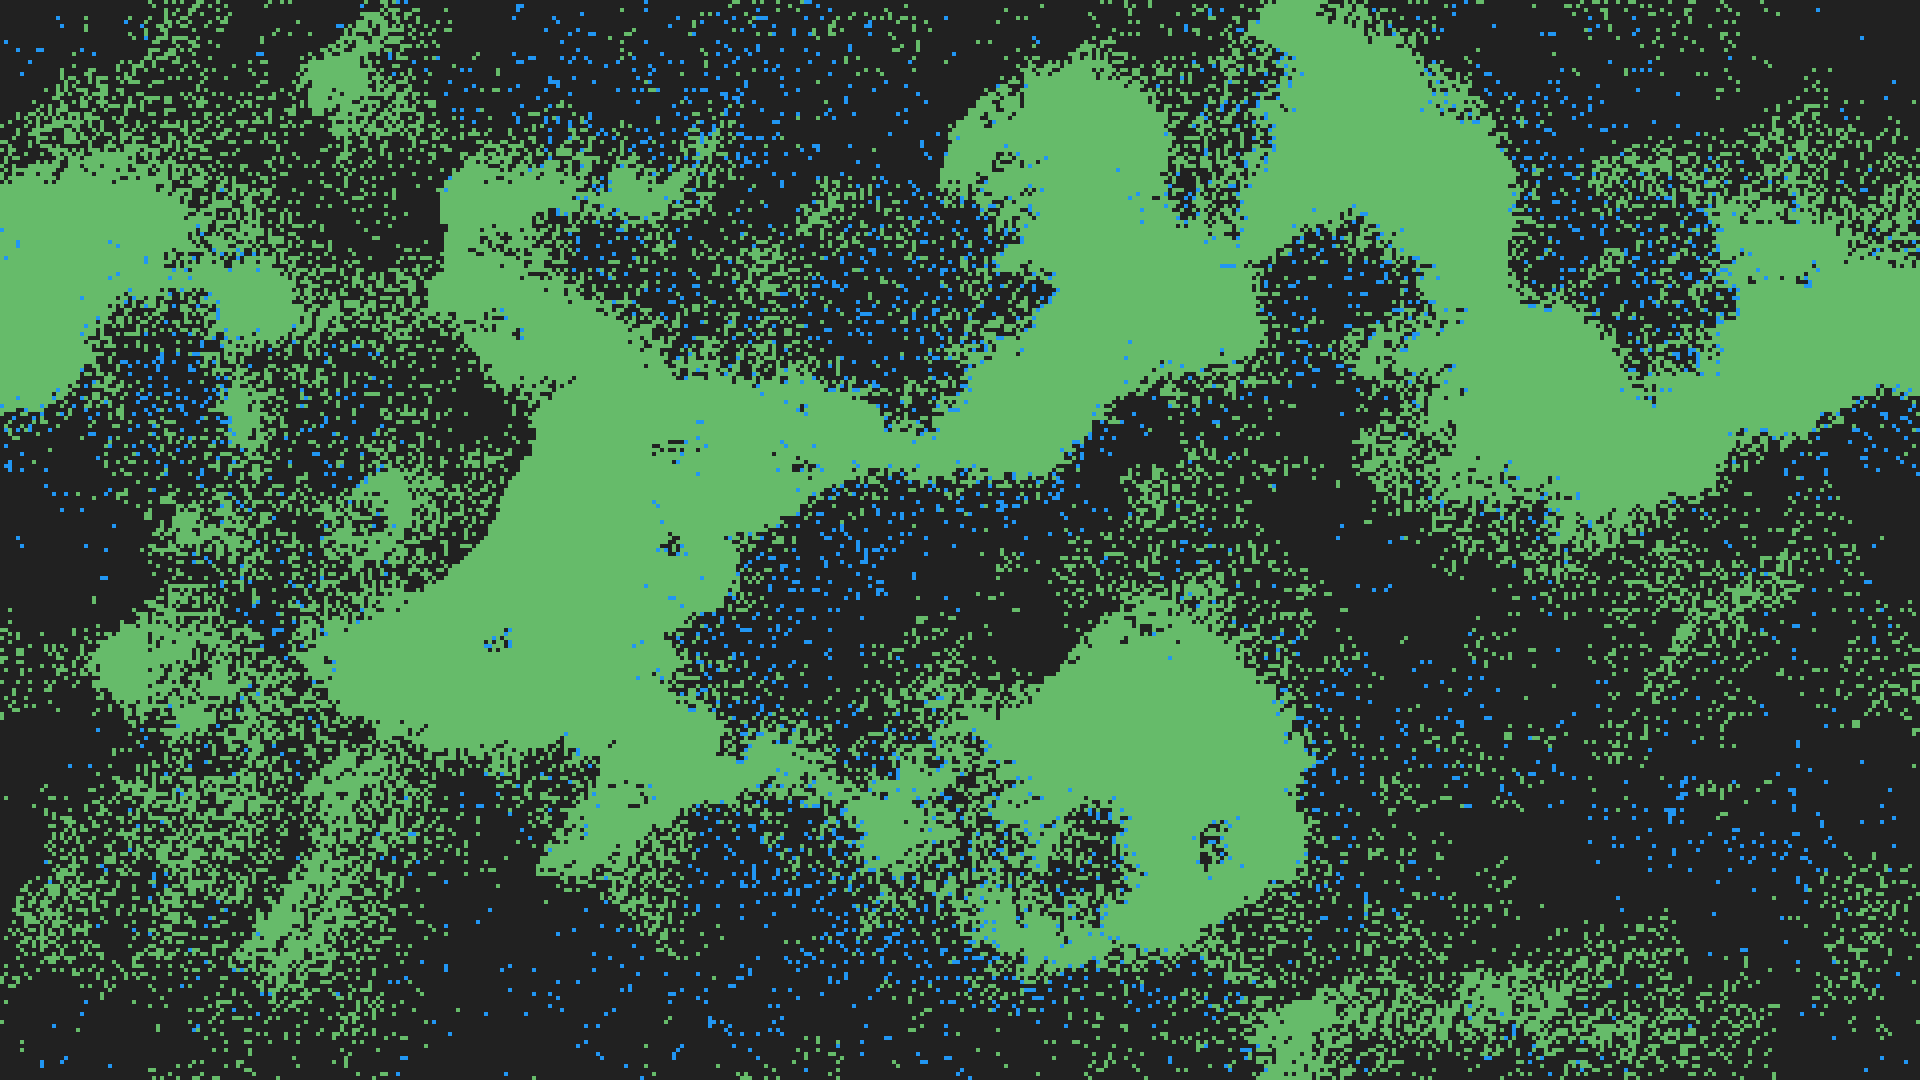
\includegraphics[width=1\textwidth]{screenshot-small.png}
	\caption{Размер на полето 480x270, 10 000 херинги и 1000 хиляди акули}
\end{figure}

\begin{figure}[H]
	\centering
	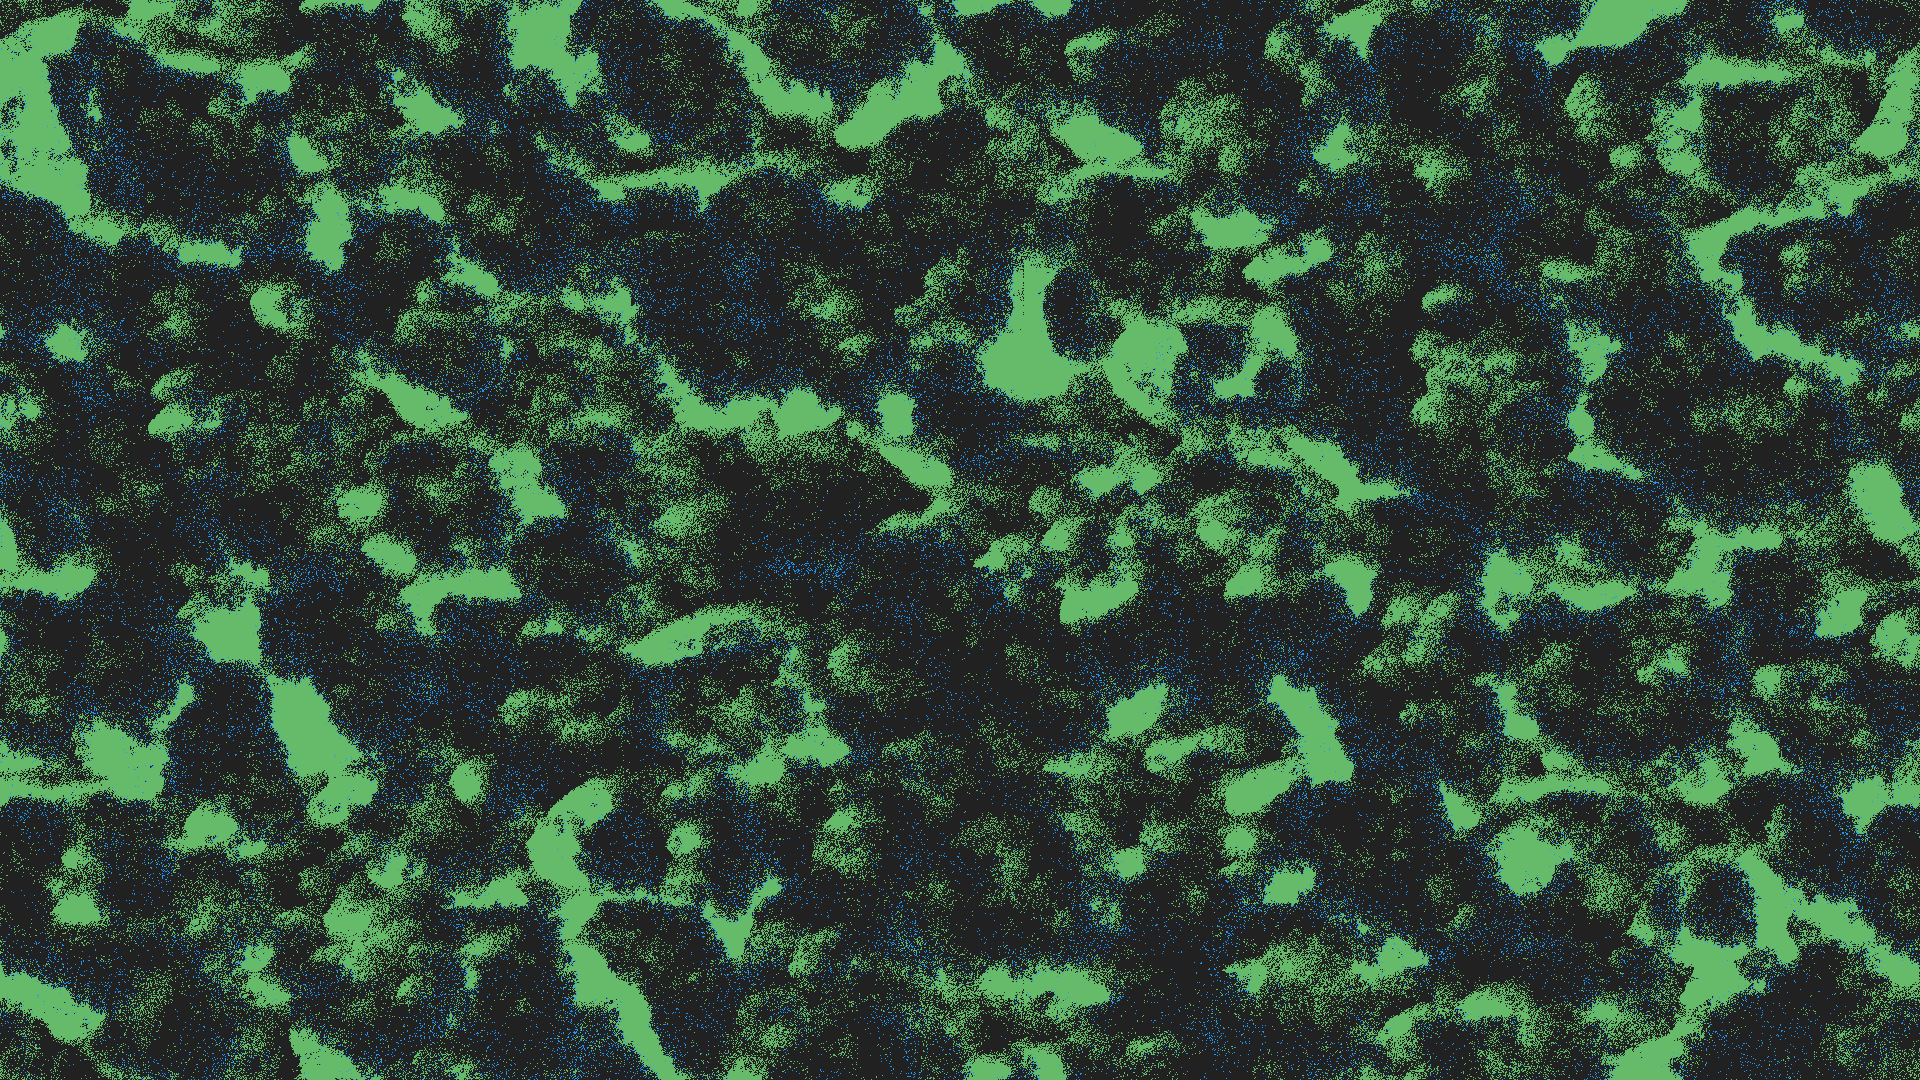
\includegraphics[width=1\textwidth]{screenshot-big.png}
	\caption{Размер на полето 1920x1080, 1 000 000 херинги и 100 000 акули}
\end{figure}

На долния линк може да бъде видяно и видео от симулацията:\\
\url{https://drive.google.com/file/d/1YTpRuH6WIVHf_kV8GkType7sPaLtN4y0/view?usp=sharing}
\bigbreak
Първоначалната цел на този "режим на работа" беше лесен начин за дебъгване,
но в крайна сметка се получи и готина анимация, която би могла да бъде доразраработена за ползване като screensaver :).

\section{Бъдещо развитие на проекта}
Резултатите, които са получени със статично балансиране са сравнително хубави,
но е възможно да се подобрят с използването на динамично балансиране на тежестта използвайки
по-фина грануларност или динамична декомпозиция на домейна. Примерен алгоритъм, който може да бъде
имплементиран в бъдеще, и да сравним резултатите с имплементацията тук
е Bounded neighbours~\cite{bounded_neighbours}, който използва динамична декомпозиция на домейна.
\bibliography{wator}{}
\bibliographystyle{plain}
\end{document}
